\Subsection{Метрические и нормированные пространства}
%BEGIN TICKET 25
\begin{definition}
    Метрика (расстояние) $\rho\!: X \times X \to [0;+\infty)$, если выполняются следующие условия:
     \begin{enumerate}
         \item $\rho(x, y) = 0 \iff x = y$,
         \item $\rho(x, y) = \rho(y, x)$,
         \item  (неравенство треугольника) $\rho(x, z) \le \rho(x, y) + \rho(y, z)$.
    \end{enumerate}
\end{definition}
\begin{definition}
    Метрическое пространство --- пара $(X, \rho)$.
\end{definition}
\begin{example}
    Дискретная метрика (метрика Лентяя) $\rho(x, y) = \begin{cases} 0, & x = y \\ 1 & x \neq y\end{cases}$
\end{example}
\begin{example}
    На $\R$:  $\rho(x, y) = |x-y|$.
\end{example}
\begin{example}
    На $\R^d$:  $\rho(x, y) = \sqrt{\sum\limits_{k=1}^d (x_k - y_k)^2}$. Неравенство треугольника здесь --- неравенство Минковского.
\end{example}
\begin{example}
    $C[a, b]$.  $\rho(f, g) = \int\limits_a^b |f-g|$.

    Неравенство треугольника:  \begin{align*}
        \rho(f, h) = \int\limits_a^b |f-h| &\overset{(*)}{\le} \int_a^b(|f-g|+|g-h|) = \rho(f, g) + \rho(g, h).\\
        (*) \iff |f(x)-h(x)| \le |f(x)-g(x)| &+ |g(x) - h(x)|\ \text{--- неравенство треугольника для }(\R, \left| x - y \right|)
    .\end{align*}
\end{example}
\begin{example}
    Манхэтеннская метрика: $\R^2$,  $\rho((x_1, y_1), (x_2, y_2)) = |x_1 - x_2| + |y_1 - y_2|$.
\end{example}
\begin{example}
    Французская железнодорожная метрика. $\R^2$. Есть точка  $P$ (Париж), тогда  $\rho(A, B) = AB$, если  $A, B,P$ на одной прямой, иначе  $\rho(A, B) = |AP|+|PB|$. 
\end{example}
\begin{definition}
    $(X, \rho)$ --- метрическое пространство.  $B_r(x) \coloneqq \{y \in X \mid \rho(x, y) < r\}$ --- открытый шар радиуса  $r$ с центром в точке  $x$. 
\end{definition}
\begin{definition}
    $(X, \rho)$ --- метрическое пространство.  $\overline{B}_r(x) \coloneqq \{y \in X \mid \rho(x, y) \le r\}$ --- закрытый шар радиуса  $r$ с центром в точке  $x$. 
\end{definition}
\begin{properties}
    \begin{enumerate}
        \item $B_{r_1}(a) \cap B_{r_2}(a) = B_{\min\{r_1, r_2\}}(a)$.
        \item $x \neq y \implies \exists r > 0\!: B_r(x) \cap B_r(y) = \emptyset \land \overline{B}_r(x) \cap \overline{B}_r(y) = \emptyset$.
    \end{enumerate}
\end{properties}
\begin{proof}
    \begin{enumerate}
        \item $x \in B_{r_1}(a) \cap B_{r_2}(a) \iff \begin{cases} \rho(x, a) < r_1 \\ \rho(x, a) < r_2 \end{cases} \iff \rho(x, a) < \min\{r_1, r_2\} \implies x \in B_{\min\{r_1, r_2\}}(a)$.
        \item $r \coloneqq \frac{1}{3} \rho(x, y) > 0$. Пусть $\overline{B}_r(x) \cap \overline{B}_r(y) \neq \emptyset$. 

            Тогда  $\exists z \in \overline{B}_r(x) \cap \overline{B}_r(y) \implies \rho(x, z) \le r \land \rho(y, z) \le r \implies \rho(x, y) \le \rho(x, z) + \rho(z, y) \le 2r = \frac{2}{3} \rho(x, y) \implies 1 \le \frac{2}{3}$. Противоречие.

            При этом, $B_r(x) \subset \overline{B}_r(x) \implies \exists r\!: B_r(x) \cap B_r(y) = \emptyset$.
    \end{enumerate}
\end{proof}
%END TICKET 25
%BEGIN TICKET 26
\begin{definition}
    $A \subset X$.  $A$ --- открытое множество, если  $\forall a \in A \exists B_r(a) \subset A$ ($r > 0$).
\end{definition}
\begin{theorem}[О свойствах открытых множеств]
    \begin{enumerate}
        \item $\emptyset, X$ --- открытые.
        \item Объединение любого числа открытых множеств --- открытое.
        \item Пересечение конечного числа открытых множеств --- открытое.
        \item $B_R(a)$ --- открытое.
    \end{enumerate}
\end{theorem}
\begin{proof}
    \begin{enumerate}
        \item[2.] $A_{\alpha}$ --- открытые,  $\alpha \in I$.  $B \eqqcolon \bigcup\limits_{\alpha \in I}A_{\alpha}$. Берем  $b \in B \implies b \in A_\beta$ для некоторого  $\beta$. Но  $A_\beta$ --- открытое  $\implies \exists r > 0\quad B_r(b) \subset A_\beta \subset B$.
        \item[3.] $A_1, A_2, \ldots, A_n$ --- открытые. $B \coloneqq \bigcap\limits_{k=1}^n A_k$. Берем  $b \in B \implies b \in A_k \forall k=1,2,\ldots,n$. Но $A_k$ --- открытое  $\implies \exists r_k > 0 B_{r_k} \subset A_k$. $\forall k\ B_{r_k}(b) \subset \bigcap\limits_{k=1}^n A_k = B \implies \exists r = \min\limits_{i = 1..k} r_k\!: B_r(b) \subset B\ \forall b \in B \implies B$ --- открытое.

         \item[4.] $\rho(a, x) < R$,  $r \coloneqq R - \rho(a, x) > 0$. Докажем, что  $B_r(x) \subset B_R(a)$. Возьмем  $y \in B_r(x)$, то есть  $\rho(x, y) < r \implies \rho(y, a) \le \rho(y, x) + \rho(x, a) < r + \rho(x, a) = R \implies y \in B_R(a)$.
    \end{enumerate}
             \begin{figure}[h!]
                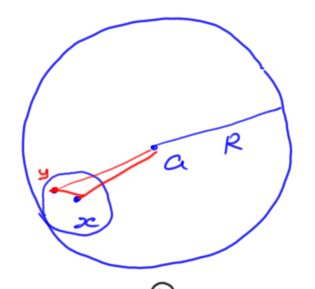
\includegraphics[width=0.25\textwidth]{open_set}
             \end{figure}
\end{proof}
\begin{remark}
    Существенна конечность. $\R$.  $\bigcap\limits_{n=1}^{\infty}(-\frac{1}{n}, 1) = [0, 1)$. А для нуля любой открытый шарик плохой.
\end{remark}
%END TICKET 26
%BEGIN TICKET 27
\begin{definition}
    $A \subset X$,  $a \in A$.  $a$ --- внутренняя точка множества  $A$, если $\exists r > 0\!: B_r(a) \subset A$.
\end{definition}
\begin{remark}
    $A$ --- открытое  $\iff$ все его точки внутренние.
\end{remark}
\begin{definition}
    Внутренность множества $\Int a \coloneqq \{ a \in A\mid a\text{ --- внутренняя точка}\}$.
\end{definition}
\begin{example}
    $A = [0, 1] \subset \R$. Тогда  $\Int A = (0, 1)$.
\end{example}
\begin{properties}[внутренности]
    \begin{enumerate}
        \item $\Int A \subset A$.
        \item  $\Int A$ ---  $\bigcup$ всех открытых множеств, которые содержатся в  $A$.
        \item $\Int A$ --- открытое множество. 
        \item  $A$ ---  открытое $\iff A = \Int A$.
        \item Если $A \subset B$, то $\Int A \subset \Int B$.
        \item $\Int(A \cap B) = \Int A \cap \Int B$
        \item $\Int(\Int A) = \Int A$.
    \end{enumerate}
\end{properties}
\begin{proof}
    \slashn
    \begin{enumerate}
        \item[2.] $B \coloneqq \bigcup_{\alpha \in I} A_{\alpha}, A_\alpha \subset A$, $A_\alpha$ открытые.

      $B \subset \Int A$. Берем  $b \in B \implies \exists \beta \in I\!: b \in A_\beta$ --- открытое  $\implies \exists r > 0\!: B_r(b) \subset A_\beta \subset A \implies b$ --- внутренняя точка  $A$  $\implies b \in \Int A$.

      $\Int A \subset B$. Берем  $b \in \Int A \implies \exists r > 0 B_r(b) \subset A$, но  $B_r(b)$ --- открытое множество $\implies $ оно участвует в объединении  $\bigcup\limits_\alpha A_\alpha \implies B_r(b) \subset B \implies b \in B$.

      \item[4.] $\Leftarrow$: пользуемся пунктом 3.  \\$\Rightarrow:$ всего его точки внутренние  $\implies A = \Int A$.

      \item[6.] $\subset$:  $A \cap B \subset A, \subset B \implies \Int(A \cap B) \subset \Int A \land \Int(A \cap B) \subset \Int B$.

      $\supset$. Пусть $x \in \Int A \cap \Int B \implies \begin{cases} \exists r_1 > 0 \quad B_{r_1}(x) \subset A \\ \exists r_2 > 0 \quad B_{r_2}(x) \subset B \end{cases} \implies$ если $r = \min \{r_1, r_2 \} \implies B_r(x) \subset A \land B_r(x) \subset B \implies B_r(x) \subset A \cap B \implies x \in \Int(A \cap B)$.

      \item[7.] $B \coloneqq \Int A$ --- открытое $\implies B = \Int B$.
    \end{enumerate}
\end{proof}
%END TICKET 27
%BEGIN TICKET 28
\begin{definition}
    $A \subset X$.  $A$ --- замкнутое, если  $X \setminus A$ --- открытое.
\end{definition}
\begin{theorem}[о свойствах замкнутых множеств]
    \begin{enumerate}
        \item $\emptyset, X$ --- замкнуты.
        \item Пересечение любого числа замкнутых множеств --- замкнуто. 
        \item Объединение конечного числа замкнутых множеств --- замкнуто.
        \item  $\overline{B}_R(a)$ --- замкнуто.
    \end{enumerate}
\end{theorem}
\begin{proof}
    \begin{enumerate}
        \item[2.] $A_\alpha$ --- замкнуты  $\implies X \setminus A_\alpha$ --- открытые  $\implies \bigcup\limits_{\alpha \in I} X \setminus A_\alpha$ --- открыто  $\implies X \setminus  \bigcup\limits_{\alpha \in I} (X \setminus A_{\alpha}) = \bigcap\limits_{\alpha \in I} A_\alpha$ --- замкнутое.
        \item[4.] $X \setminus \overline{B}_R(a)$ --- открытое. Берем  $x \notin \overline{B}_R(a)$. Возьмем $r \coloneqq \rho(a, x) - R > 0$. Покажем, что  $B_r(x) \subset X \setminus \overline{B_R}(a)$.

            От противного. Пусть $B_r(x) \cap \overline{B}_R(a) \neq \emptyset$. Берем  $y \in B_r(x) \cap \overline{B}_R(a) \implies \rho(x, y) < r \land \rho(a, y) \le R \implies \rho(a, x) \le \rho(a, y) + \rho(y, x) < R + r = \rho(a, x)$. Противоречие.
    \end{enumerate}
\end{proof}
\begin{remark}
    В 3 важна конечность. $\R$.  $\bigcup\limits_{n=1}^{\infty} [\frac{1}{n}, 1] = (0, 1]$ --- не является замкнутой.
\end{remark}
\begin{definition}
    Замыкание множества $\Cl A$ --- пересечение всех замкнутых множеств, содержащих  $A$.
\end{definition}
\begin{theorem}
    $X \setminus \Cl A = \Int(X \setminus A)$ и  $X \setminus \Int A = \Cl(X \setminus A)$.
\end{theorem}
\begin{proof}
    $\Int(X \setminus A) = \bigcup B_{\alpha}$.  $B_\alpha$ --- открытые,  $B_\alpha \subset X \setminus A \iff X \setminus B_\alpha$ --- замкнутое. $X \setminus B_\alpha \supset A$.

    $\bigcap(X \setminus B_\alpha) = \Cl A \implies X \setminus \bigcap (X \setminus B_\alpha) = X \setminus \Cl A \iff \bigcup(B_\alpha) = \Int(X \setminus A)$.
\end{proof}
\begin{consequence}
    $\Int A = X \setminus Cl(X \setminus A)$ и  $\Cl A = X \setminus \Int(X \setminus A)$.
\end{consequence}
\begin{properties}
    \begin{enumerate}
        \item $\Cl A \supset A$.
        \item  $\Cl A$ --- замкнутое множество. 
        \item $A$ --- замкнуто  $\iff A = \Cl A$.
            \begin{proof}
                $\Leftarrow$ --- пункт 2.  $\Rightarrow A$ --- замкнутое  $\Rightarrow$ оно участвует в пересечении из определения  $\implies \Cl A \subset A \implies \Cl A = A$.
            \end{proof}
        \item $A \subset B \implies \Cl A \subset \Cl B$.
             \begin{proof}
                $X \setminus A \supset X \setminus B \implies \Int(X \setminus A) \supset \Int(C \setminus B) \implies X \setminus \Int(X \setminus A) \subset X \setminus \Int(X \setminus B)$
            \end{proof}
        \item $\Cl(A \cup B) = \Cl A \cup \Cl B$.
        \item  $\Cl(\Cl A) = \Cl A$.
             \begin{proof}
                $B \coloneqq \Cl A$ --- замкнуто  $\implies \Cl B = B$.
            \end{proof}
    \end{enumerate}
\end{properties}
\begin{exerc}
    $\Cl \Int \Cl \Int \ldots A$. Какое наибольшее количество различных множеств может получиться.
\end{exerc}
\begin{theorem}
    $x \in \Cl A \iff \forall r > 0\quad B_r(x) \cap A \neq \emptyset$.
\end{theorem}
\begin{proof}
    Запишем отрицание условия теоремы: $x \notin \Cl A \iff \exists r > 0 B_r(x) \cap A = \emptyset$.

    Что означает, что  $x \notin A$? Это значит, что  $x\in X \setminus \Cl A = \Int(X \setminus A) \iff x \in \Int(X \setminus A) \iff x\text{ --- внутренняя точка }X \setminus A \iff \exists r > 0\!: B_r(x) \cap A = \emptyset \iff \exists r > 0\!: B_r(x) \subset X \setminus A$.
\end{proof}
\begin{consequence}
    $U$ --- открытое,  $U \cap A = \emptyset \implies U \cap \Cl A = \emptyset$.
\end{consequence}
\begin{proof}
    Возьмем $x \in U \implies \exists r > 0\!: B_r(x) \subset U \implies B_r(x) \cap A = \emptyset \implies x \notin \Cl A \implies U \cap \Cl A = \emptyset$.
\end{proof}
%END TICKET 28
%BEGIN TICKET 29
\begin{definition}
    Окрестностью точки $x$ будем называть шар  $B_r(x)$ для некоторого  $r > 0$. Обозначать будем $U_x$
\end{definition}
\begin{definition}
    Проколотой окрестностью точки $x$ ---  $B_r(x) \setminus \{x\}$. Обозначать будем $\dot{U}_x$.
\end{definition}

\begin{definition}
    $x$ --- предельная точка множества  $A$, если  $\forall \dot{U_x}\!: \dot{U_x} \cap A \neq \emptyset$.

    Обозначим через  $A'$ --- множество предельных точек для  $A$.
\end{definition}
\begin{properties}
    \slashn
    \begin{enumerate}
        \item $\Cl A = A \cup A'$.
            \begin{proof}
                $x \in \Cl A \iff \forall U_x\!: U_x \cap A \neq \emptyset \iff \left[ \begin{array}{l} x \in A \\ \forall \dot{U_x} \cap A \neq \emptyset \iff x \in A' \end{array} \right.$
            \end{proof}
        \item $A \subset B \implies A' \subset B'$. Очевидно.
        \item  $A$ --- замкнуто  $\iff A \supset A'$. 
             \begin{proof}
                $A$ --- замкнуто  $\iff A = \Cl A \iff A = A \cup A' \iff A \supset A'$.
            \end{proof}
        \item $(A \cup B)' = A' \cup B'$.
             \begin{proof}
                Докажем "$\subset$". Возьмем $x \in (A \cup B)'\!: x \notin A' \implies \exists \dot{U_x}\!: \dot{U_x} \cap A = \emptyset$, но $\dot{U_x} \cap (A \cup B) \neq \emptyset \implies \dot{U_x} \cap B \neq \emptyset \implies x \in B'$.

                Докажем "$\supset$". $A \cup B \supset A \implies (A \cup B)' \supset A'$. Провернем тот же фокус для  $B$, получим  $(A \cup B)' \supset A' \cup B'$.
           \end{proof}
    \end{enumerate}
\end{properties}
\begin{theorem}
    $x \in A' \iff \forall r > 0$  $B_r(x)$ содержит бесконечное количество точек из  $A$.
\end{theorem}
\begin{proof}
    Докажем "$\Leftarrow$". $B_r(x) \cap A$ содержит бесконечное количество точек  $\implies \dot{B_r}(x) \cap A$ содержит бесконечное число точек  $\implies \dot{B_r}(x) \cap A \neq \emptyset \Rightarrow x \in A'$.

     "$\Rightarrow$". Возьмем радиус  $r$. Тогда  $\dot{B_r}(x) \cap A \neq \emptyset \implies \exists x_1 \in A\!: 0 < \rho(x, x_1) < r$. Возьмем $r = \rho(x, x_1)$ $\dot{B_r}(x) \cap A \neq \emptyset \implies \exists x_2 \in A\!: 0 < \rho(x, x_2) < \rho(x, x_1)$. Тогда можно взять $r = \rho(x, x_2)$, и так далее. 

     В итоге получили, что $r > \rho(x, x_1) > \rho(x, x_2) > \rho(x, x_3) > \ldots > 0 \implies$ все $x_n$ различны.
\end{proof}
\begin{consequence}
     Конечное множество не имеет предельных точек.
\end{consequence}
\begin{proof}
     Предположим предельная точка существует $\iff \exists r > 0\!: B_r(x) \cap A$ содержит бесконечное количество точек. Но это невозможно, так как в $A$ конечное число точек.
\end{proof}
%END TICKET 29
%BEGIN TICKET 30

\begin{definition}
     $(X, \rho)$ --- метрическое пространство  $Y \subset X$.

     Тогда  $(Y, \rho \mid_{Y \times Y})$ --- подпространство метрического пространства  $(X, \rho)$.
\end{definition}
\begin{example}
     $(\R, |x-y|)$.  $Y=[a, b] \subset \R$, например, $Y=[0, 1]$.

      $B_1(1) = (0, 1], B_2(0) = [0, 1]$.  $B_r^Y(a) = Y \cap B_r^X(a)$. ($B^A_r -$ шарик радиуса $r$ на множестве $A$)
\end{example}
\begin{theorem}[об открытых и замкнутых множества в пространстве и подпространстве]
     $(X, \rho)$ --- метрическое пространство,  $(Y, \rho)$ --- его подпространство,  $A \subset Y$. Тогда
      \begin{enumerate}
          \item $A$ --- открыто в  $Y \iff \exists G$ --- открытое в  $X\!: A = G \cap Y$. 
          \item $A$ --- замкнуто в  $Y \iff \exists F$ --- замкнутое в  $X\!: A = F \cap Y$.
     \end{enumerate}
\end{theorem}
\begin{proof}
     \slashn
     \begin{enumerate}
         \item "$\Rightarrow$" $A$ --- открыто в  $Y \implies \forall x \in A \exists r_x > 0 \!: B_{r_x}^Y(x) \subset A \implies A = \bigcup\limits_{x \in A}B_{r_x}^Y(x)$.

             То есть наше множество будет объединением большего числа шариков (возможно бесконечного). Найдем теперь  $G$:  $G \coloneqq \bigcup\limits_{x \in A} B_{r_x}^X(x)$ --- открыто. Посмотрим теперь на  $G \cap Y = \bigcup\limits_{x \in A}(B_{r_x}^X(x) \cap Y) = \bigcup\limits_{x \in A}B_{r_x}^Y(x) = A$.

         В обратную сторону. Пусть $A = G \cap Y$, где  $G$ открыто в  $X$. Возьмем  $x \in G \cap Y$.  $G$ --- открыто в  $X \implies \forall x \in G \cap Y \exists r > 0\!: B_r^X(x) \subset G \implies B_r^X(x) \cap Y \subset G \cap Y = A \implies B_r^Y(x) \subset A \implies x$ --- внутренняя точка $A \implies A$ --- открыто в  $Y$. 

         \item $A$ --- замкнуто в $Y \iff Y \setminus A$ --- открыто в  $Y \iff \exists G$ --- открытое в  $X$, такое что  $Y \setminus A = Y \cap G \iff A = Y \setminus (Y \cap G) \overset{(1)}{=} Y \setminus G \overset{(2)}{=} Y \cap (X \setminus G) \iff \exists G$ --- открытое в  $X$, такое что  $A = Y \cap (X \setminus G) \iff \exists F$ --- замкнуто в  $X$, такое что  $A = Y \cap F$.

             $(1)$ --- Можно забить на пересечение с  $Y$, потому что, если элемент  $G$ не лежит в $Y$, то и в $Y \setminus G$ он участия не принимает.  $(2)$ --- Помним, что  $Y \subset X$, а значит такая операция корректна.
     \end{enumerate}
\end{proof}
\begin{example}
     $(\R, |x-y|)$.  $Y = [0, 3)$.  $[0, 1)$ --- открыто в  $[0, 3)$:  $[0, 1) = [0, 3) \cap (-1, -1)$.  $[2, 3)$ --- замкнуто в  $[0, 3)$:  $[2, 3) = [0, 3) \cap [2, 3]$.
\end{example}
 
%END TICKET 30
%BEGIN TICKET 31
\begin{definition}
     $X$ --- векторное пространство над  $\R$.

      $||.||\!: X \to \R$ --- норма, если
       \begin{enumerate}
           \item $||x|| \ge 0\quad \forall x \in X$ и $||x|| = 0 \iff x = \overrightarrow{0}$.
           \item  $||\lambda x|| = |\lambda| \cdot ||x||\quad \forall x \in X\ \forall \lambda \in \R$. 
           \item (неравенство треугольника)
      \end{enumerate}
\end{definition}
\begin{example}
     \begin{enumerate}
         \item $|x| \in \R$,
         \item  $||x||_1 = |x_1| + |x_2| + \ldots + |x_d|$ в $\R^d$.
         \item  $||x||_{\infty} = \max\limits_{k=1,2,\ldots, d} |x_k|$. $||x+y||_{\infty} = \max\{|x_k|+|y_k|\} \le \max\{|x_k|\} + \max\{|y_k|\} = ||x||_{\infty} + ||y||_{\infty}$
         \item $||x||_2 = \sqrt{x_1^2 + x_2^2 + \ldots + x_n^2}$.
         \item $||x||_p = \left(\sum\limits_{k=1}^d |x_k|^p\right)^{\frac{1}{p}}$ в $\R^d$ при  $p \ge 1$. Неравенство треугольника --- неравенство Минковского.
         \item $C[a, b]$.  $||f|| = \max\limits_{t \in [a, b]} |f(t)|$. 
     \end{enumerate}
\end{example}
\begin{definition}
    $X$ векторное пространство над  $\R$.  $\langle .,.\rangle\!: X \times X \to \R$ скалярное произведение, если
     \begin{enumerate}
         \item $\langle x, x \rangle \ge 0$ и $\langle x, x \rangle = 0 \iff x = \overrightarrow{0}$.
         \item  $\langle x+y, z\rangle = \langle x, z \rangle + \langle y, z \rangle$
         \item  $\langle x, y \rangle = \langle y, x \rangle$.
         \item  $\langle \lambda x, y \rangle = \lambda \langle x, y \rangle \quad \lambda \in \R$.
    \end{enumerate}
\end{definition}
\begin{example}
    \begin{enumerate}
        \item $\R^d$.  $\langle x, y\rangle = \sum x_iy_i$.
        \item Возьмем $w_1, \ldots, w_d > 0$. Тогда $\langle x, y \rangle = \sum w_i x_i y_i$.
        \item $C[a, b]$.  $\langle f, g \rangle = \int\limits_a^b f(x)g(x) \mathrm{d}x$.
    \end{enumerate}
\end{example}
\begin{properties}
    \begin{enumerate}
        \item Неравенство Коши-Буняковского. $\langle x, y \rangle^2 \le \langle x, x \rangle \cdot \langle y, y\rangle$.
            \begin{proof}
                $f(t) \coloneqq \langle x+ty, x +ty \rangle \ge 0$. $f(t) = \langle x, x \rangle + t\langle x, y \rangle + t\langle x, y \rangle + t^2 \langle y, y \rangle = t^2 \langle y, y\rangle + 2t\langle x, y \rangle + \langle x, y \rangle$ --- квадратный трехчлен (если $\langle y, y \rangle = 0 \implies y = 0 \implies$ везде нули). Тогда $0 \ge D= (\langle x, y \rangle)^2 - 4 \langle x, x\rangle \cdot \langle y, y \rangle = 4(\langle x, y \rangle^2 - \langle x, x\rangle \cdot \langle y, y \rangle)$. Потому что иначе есть два корня и где-то есть отрицательное значение, а $f(t) \geq 0$.
            \end{proof}
        \item $||x|| \coloneqq \sqrt{\langle x, x \rangle}$ --- норма.
             \begin{proof}
                $||\lambda x|| = \sqrt{\langle \lambda x, \lambda x\rangle} = \sqrt{\lambda^2\langle x, x \rangle} = |\lambda| \sqrt{\langle x, x \rangle} = |\lambda| \cdot ||x||$.

                Неравенство треугольника: $\lVert x+y \rVert \le \lVert x \rVert + \lVert y \rVert$.
                Возведем в квадрат, получим $\langle x + y, x + y\rangle \le \langle x, x\rangle + \langle y, y\rangle + 2\sqrt{\langle x, x\rangle\langle y, y\rangle}$, но теперь вспомним, что $\langle x + y, x + y\rangle = \langle x, x\rangle + \langle y, y\rangle + 2\langle x, y\rangle$.
                А, сократив общие слагаемые, получим доказанное неравенство Коши-Буняковского.
            \end{proof}
        \item $\rho(x, y) = \lVert x - y \rVert$ --- метрика.
            \begin{proof}
                $\rho(x, y) \ge 0$. $\rho(x, y) = 0 \iff \lVert x - y \rVert = 0 \iff x - y = \overrightarrow{0} \iff x = y$.

                 $\rho(y, x) = \lVert y-x \rVert = \lVert (-1)(x-y) \rVert = |-1| \lVert x - y \rVert = \rho(x, y)$.

                  $\rho(x, z) \le \rho(x, y) + \rho(y, z)$: $\lVert (x-y) + (y-z) \rVert = \lVert x-z\rVert \le \lVert x - y \rVert + \lVert y-z \rVert$.
            \end{proof}
        \item $\lVert x - y \rVert \ge |\lVert x \rVert - \lVert y \rVert |$.
            \begin{proof}
                Надо доказать, что $-\lVert x - y \rVert \le \lVert x \rVert - \lVert y \rVert \le \lVert x - y \rVert$.

                Левое: $\lVert y \rVert = \lVert (y - x) + x \rVert \le \lVert y - x \rVert + \lVert x \rVert$

                Правое: $\lVert x \rVert = \lVert (x - y) + y \rVert \le \lVert x - y \rVert + \lVert y \rVert$

            \end{proof}
        \item Упражненение. Если норма порождается скалярным произведением $\iff \lVert x+y\rVert^2 + \lVert x-y\rVert^2 = 2\lVert x\rVert^2 + 2\lVert y \rVert^2$. Тождество параллелограмма.
    \end{enumerate}
\end{properties}
\begin{definition}
    $(X, \rho)$ --- метрическое пространство.  $x_1, x_2, \ldots \in X, a \in X$.

    $\lim x_n = a$, если
     \begin{enumerate}
         \item Вне любого открытого шара с центром в точке  $a$ содержится лишь конечное число членов последовательности.
         \item  $\forall \eps > 0 \exists N \forall n \ge N\quad \rho(x_n, a) < \eps \iff x_n \in B_\eps(a)$.
    \end{enumerate}
\end{definition}
\begin{definition}
    $A \subset X$. 

    Тогда  $A$ --- ограничено, если оно содержится в некотором шаре.
\end{definition}
\begin{properties}
    \begin{enumerate}
        \item $a = \lim x \iff \rho(x_n, a) \to 0$.
\begin{proof}
             $\forall \eps > 0 \exists n > N\quad |\rho(x_n, a)| < \eps$ --- предел равен 0.
\end{proof}
        \item Предел единственный. 
            \begin{proof}
                Пусть $a = \lim x_n$ и $b = \lim x_n$. Тогда возьмем шарики такие, что  $B_r(a) \cap B_r(b) = \emptyset \implies \exists N_1, N_2, \forall n \ge \max\{N_1, N_2\} x_n \in B_r(a) \land x_n \in B_r(b)$ --- противоречие.
            \end{proof}
        \item Если $a = \lim x_n, a = \lim y_n$. То для перемешанной последовательности $x_n$ и  $y_n$ предел такой же.
        \item  $a = \lim x_n \implies $ для последовательности, в которой $x_n$ взяты с конечной кратностью, $a$ будет пределом.
        \item Если $a = \lim x_n$, то  $\lim x_{n_k} = a$.
        \item Последовательность имеет предел $\implies$ она ограничена
             \begin{proof}
                $\eps = 1 \exists N \forall n \ge N \rho(x_n, a) < 1$. Тогда $R = \max\{\rho(x_1, a), \ldots, \rho(x_{N-1}, a)\} + 1 \implies x_n \in B_R(a)$.
            \end{proof}
        \item Если $a = \lim x_n$, то последовательность, полученная из  $\{x_n\}$ перестановкой членов имеет тот же предел.
        \item $a$ --- предельная точка  $A \iff \exists \{x_n\} \neq a \in A\!: \lim x_n = a$.

            Более того,  $x_n$ можно выбирать так, что  $\rho(x_n, a)$ строго убывает.
            \begin{proof}
                "$\Rightarrow$" Пусть  $\lim x_n = a$. Возьмем  $B_r(a) \implies \exists N \forall n \ge N x_n \in B_r(a) \implies x_n \in \dot{B_r}(a) \implies \dot{B_r}(a) \cap A \neq \emptyset \implies$ a --- предельная точка.

                "$\Leftarrow$" Берем  $r_1 = 1$. $\dot{B_{r_1}}(a) \cap A \neq \emptyset$. Берем оттуда точку, называем  $x_1 \neq a$. $r_2 = \frac{\rho(x_1,a)}{2}$. $\dot{B_{r_2}}(a) \cap A \neq \emptyset$. Берем оттуда точку $x_3 \neq a$. $r_3 = \frac{\rho(x_2, a)}{2}$. И так далее.

                Получили: $x_n \neq a$ и  $\rho(x_n, a) < \frac{\rho(x_{n-1}, a)}{2} < \rho(x_{n-1}, a)$. $\rho(x_n, a) < \frac{1}{2^n} \to 0 \implies x_n = a$.
            \end{proof}
    \end{enumerate}
\end{properties}
\begin{theorem}[об арифметических действиях с пределами]
    $X$ --- нормированное пространство,  $x_n, y_n \in X$,  $\lambda_n \in \R$.  $\lim x_n = a, \lim y_n = b, \lim \lambda_n = \mu$. Тогда:
     \begin{enumerate}
         \item $\lim (x_n + y_n) = a+b$.
         \item  $\lim(x_n - y_n) = a-b$.
         \item  $\lim \lambda_nx_n = \mu a$.
         \item  $\lim \lVert x_n\rVert = \lVert a \rVert$.
         \item  Если в  $X$ есть скалярное произведение, то  $\lim \langle x_n, t_n \rangle = \langle a, b \rangle$.
    \end{enumerate}
\end{theorem}
\begin{proof}
    \begin{enumerate}
        \item $\rho(x_n+y_n, a+b) = \lVert (x_n+y_n - (a+b)) \rVert = \lVert (x_n-a) + (y_n-b) \rVert \le \lVert x_n - a \rVert + \lVert y_n - n \rVert = \rho(x_n, a) + \rho(y_n, b) \to 0$.
        \item Аналогично.
        \item $\rho(\lambda_nx_n, \mu a) = \lVert \lambda_n x_n - \mu a\rVert = \lVert \lambda_n x_n - \lambda_n a + \lambda_n a - \mu a \rVert \le \lVert \lambda_n x_n - \lambda_n a \rVert + \lVert \lambda_n a - \mu a \rVert = |\lambda_n| \lVert x_n - a \rVert + |\lambda_n -\mu| \lVert a \rVert \to 0$, так как $|\lambda_n|$ --- ограниченная, $\lVert x_n - a \rVert = \rho(x_n - a) \to 0$,  $|\lambda_n -\mu| \to 0$, $\lVert a \rVert$ --- константа.  
        \item $| \lVert x_n \rVert - \lVert a \rVert| \le \lVert x_n - a \rVert = \rho(x_n, a) \to 0 \implies \lim \lVert x_n \rVert = \lVert a \rVert$
        \item $\langle x, y \rangle = \frac{1}{4}(\lVert x+y \rVert^2 - \lVert x-y \rVert^2) = \frac{1}{4}(\langle x+y, x+y\rangle - \langle x-y, x-y\rangle)$. Тогда получаем $4 \langle x_n, y_n \rangle = \lVert x_n + y_n \rVert^2 - \lVert x_n - y_n \rVert^2 \to \lVert a + b \rVert^2 - \lVert a - b \rVert^2 = 4 \langle a, b \rangle$.
    \end{enumerate}
\end{proof}
\begin{definition}
    $\R^d$ --- пространство с нормой  $\sqrt{x_1^2 + x_2^2 + \ldots + x_d^2}$.
\end{definition}
\begin{definition}
    Покоординатная сходимость в $R^d$:

    $x_n \in \R^d$.  $x_n = (x_n^{(1)}, x_n^{(2)}, \ldots, x_n^{(d)}) \xrightarrow{\text{покоординатно}} a = (a^{(1)}, a^{(2)}, \ldots, a^{(d)})$.
\end{definition}
\begin{theorem}
    в $\R^d$ сходимость по метрике и покоординатная сходимость совпадает.
\end{theorem}
\begin{proof}
    Метрика $\implies$ покоординатная.  $\rho(x_n, a) \to 0 \implies 0 \le (x_n^{(1)} - a^{(1)})^2 + \ldots + (x_n^{(d)} - a^{(d)})^2 = \rho(x_n, a)^2 \to 0 \implies \lim (x_n^{(k)} - a^{(k)})^2 = 0 \implies \lim x_n^{(k)} = a^{(k)} \implies$ покоординатная сходимость.

    Покоординатная $\implies$ метрика. Пусть  $|x_n^{(k)} - a^{(k)}| \to 0 \quad \forall k \implies (x_n^{(k)} - a^{(k)})^2 \to 0 \implies \sum\limits_{k=1}^d (x_n^{(k)} - a^{(k)})^2 \to 0$. А так как $(\ldots)^2 = \rho(x_n, a)^2 \implies \rho(x_n, a) \to 0$.
\end{proof}

\begin{definition}
    $x_n \in X$ --- фундаментальная последовательность, если
     \[
    \forall \eps > 0 \exists N \forall m, n \ge N\!: \rho(x_n, x_m) < \eps
    .\] 
\end{definition}
\begin{properties}
    \begin{enumerate}
        \item Сходящаяся последовательность фундаментальна.
        \item Фундаментальная последовательность ограничена.
        \item Если у последовательности есть сходящаяся подпоследовательность, то последовательность имеет предел.
    \end{enumerate}
\end{properties}
\begin{proof}
    Упражнение! Утверждается, что так же, как и в пределах.
\end{proof}
\begin{definition}
    $(x, \rho)$ --- метрическое пространство --- полное, если любая фундаментальная последовательность имеет предел.
\end{definition}
\begin{example}
    $\R\!:$,  $\rho(x, y) = |x-y|$ --- полное.
\end{example}
\begin{exerc}
    $(X, \rho)$ --- полное метрическое пространство  $X \supset Y$ замкнуто. Доказать, что  $(Y, \rho)$ --- полное.
\end{exerc}
\begin{exerc}
    $(0, 1)$ не полное.  $x_n = \frac{1}{n}$ --- фундаментальная, но $\lim \frac{1}{n} = 0 \notin (0; 1)$.
\end{exerc}
\begin{theorem}
    $\R^d$ --- полное.
\end{theorem}
\begin{proof}
    Пусть $x_n$ --- фундаментальная, то есть
     \[
    \forall \eps > 0 \exists N \forall m,n \ge N\!: \rho(x_n, x_m) = \sqrt{(x_n^{(1)}-x_m^{(1)})^2 + \ldots + (x_n^{(d)}-x_m^{(d)})^2} < \eps
    .\] 

    Но мы знаем, что $\rho(x_n, x_m) \ge |x_n^{(k)} - x_m^{(k)}|$. Тогда заметим, что $x_n^{(k)}$ --- фундаментальная  $\implies \exists a^{(k)} = \lim\limits_{n \to \infty} x_n^{(k)}$. Значит и  $x_n$ сходится к  $a$ покоординатно  $\implies \rho(x_n, a) \to 0 \implies x_n$ сходится к  $a$ по метрике.
\end{proof}
\Subsection{Компактность}
\begin{definition}
    $A, U_\alpha, \alpha \in I$.

    Множества  $U_\alpha$ --- покрытие множества  $A$, если  $A \subset \bigcup\limits_{\alpha \in I} U_\alpha$.
\end{definition}
\begin{definition}
    Открытое покрытие --- покрытие открытыми множествами.
\end{definition}
\begin{definition}
    $(X, \rho)$ --- метрическое пространство, $K \subset X$.

    $K$ --- компакт, если из любого его открытого покрытия можно выделить конечное подпокрытие. 
\end{definition}
\begin{definition}
    То есть для любого покрытия можно выбрать $\alpha_1, \alpha_2, \ldots, \alpha_n \in I\!: K \subset\bigcup \limits_{i=1}^n U_{\alpha_i}$
\end{definition}
\begin{theorem}[Теорема о свойствах компактных множеств]
    \begin{enumerate}
        \item $K \subset Y \subset X$. Тогда  $K$ --- компакт в  $(X, \rho) \iff K$ --- компакт в  $(Y, \rho)$.
        \item  $K$ --- компакт  $\implies K$ замкнуто и ограничено.
        \item  Замкнутое подмножество компакта --- компакт.
    \end{enumerate}
\end{theorem}
\begin{proof}
    \begin{enumerate}
        \item $\Leftarrow$. Пусть  $G_\alpha$ покрытие  $K$ множествами, открытыми в $X$. Тогда  $U_\alpha = G_\alpha \cap Y$ --- открыты в  $Y$ и $K \subset \bigcup_{\alpha \in I} U_\alpha = \bigcup_{\alpha \in I} G_\alpha \cap Y = (\bigcup_{\alpha \in I} G_\alpha) \cap Y$.

             $U_\alpha$ --- открытое покрытие в  $(Y, \rho) \implies$ можно выделить конечное подпокрытие  $\alpha_1, \ldots, \alpha_n$, такое что $K \subset \bigcup\limits_{i=1}^n U_{\alpha_i} \subset \bigcup\limits_{i=1}^n G_{\alpha_i}$ --- конечное подпокрытие $G_\alpha \implies K$ компакт в  $(X, \rho)$.

              $\Rightarrow$. Воспользуемся тем же наблюдением: $U_\alpha = G_\alpha \cap Y$. Следовательно можно выбрать  $\alpha_1, \alpha_2, \ldots, \alpha_n$ в $X$ и они же подойдут и в  $Y$. 
          \item Ограниченность. Возьмем $a \in X$. Тогда  $K \subset \bigcup\limits_{n=1}^\infty B_n(a) = X$ --- открытое покрытие  $K$. Выделим конечное подпокрытие  $K \subset \bigcup\limits_{n=1}^N B_n(a) \implies K \subset B_N(a) \implies K$ --- ограничено. 

              Замкнутость. Надо доказать, что $X \setminus K$ --- открытое. Возьмем  $a \in X \setminus K$ и $x \in K$ и докажем, что  $a$ лежит в  $X \setminus K$ вместе с некоторым шариком.

              Пусть  $U_x = B_{\frac{\rho(x, a)}{2}}(x)$. Причем он не пересекается с $B_x = B_{\frac{\rho(x, a)}{2}}(a)$. Возьмем тогда $K \subset \bigcup_{x \in K} U_x$ --- открытое покрытие (поскольку каждый шарик точно покрывает свой центр и ещё что-то). Выделим конечное подпокрытие  $K \in \bigcup\limits_{i=1}^n U_{x_i}$,  $r = \min\{\frac{\rho(x_i, a)}{2} \}$. Тогда $B_r(a) = \bigcap\limits_{i=1}^n B_{x_i}$.  $B_r(a) \cap \bigcup\limits_{i=1}^n U_{x_i} = \emptyset \implies B_r(a) \cap K = \emptyset \implies B_r(a) \subset X \setminus K \implies a$ --- внутренняя $X \cap K$.
          \item Пусть $\widetilde{K}$ --- компакт,  $K$ --- замкнуто и  $K \subset \widetilde{K}$.

              Рассмотрим открытое покрытие  $K$  $U_\alpha$. Тогда  $\widetilde{K}$ покрыто  $(X \setminus K) \cup \bigcup\limits_{\alpha \in I} U_\alpha$ -- открытое покрытие  $\widetilde{K}$. Выделим конечное подпокрытие  $X \setminus K, U_{\alpha_1}, \ldots, U_{\alpha_n}$. $K \subset X \setminus K \cup \bigcup\limits_{i=1}^n U_{\alpha_i} \implies K \subset \bigcup\limits_{i=1}^n U_{\alpha_i}$ --- открытое множество, а значит  $K$ --- компакт.
    \end{enumerate}
\end{proof}
\begin{theorem}
    $K_\alpha$ --- семейство компактов, такое что пересечение любого конечного числа из них непусто. Тогда  $\bigcap_{\alpha \in I} K_\alpha \neq \emptyset$.
\end{theorem}
\begin{consequence}
    $K_1 \subset K_2 \subset K_3 \subset \ldots$ непустые компакты. Тогда $\bigcap\limits_{n=1}^\infty K_n \neq \emptyset$.
\end{consequence}
\begin{proof}
    От противного. Пусть $\bigcap\limits_{\alpha \in I} K_\alpha = \emptyset$. Зафиксируем компакт  $K_0 \implies K_0 \cap \bigcap\limits_{\alpha \in I} K_\alpha = \emptyset \implies K_0 \subset X \setminus \bigcap\limits_{\alpha \in I} K_\alpha = \bigcup_{\alpha \in I} X \setminus K_\alpha$ --- открытое покрытие  $K_0$. Выделим конечное подпокрытие  $K_0 \subset \bigcup\limits_{i=1}^n X \setminus K_{\alpha_i} = X \setminus \bigcap\limits_{i=1}^n K_{\alpha_i} \implies K_0 \cap \bigcap\limits_{i=1}^n K_{\alpha_i} = \emptyset$.??!
\end{proof}

\begin{definition}
    $K$ --- секвенциально компактное множество, если из любой последовательности точек из $K$ можно выделить подпоследовательность, которая сходится к какой-то точке из  $K$.
\end{definition}
\begin{example}
    $[a, b] \in \R$ секвенциально компактно.

     $x_n \in [a; b] \xRightarrow{\text{Т. Б-В}} \exists$ подпоследовательность $x_{n_k}$, имеющая предел  $\implies \lim x_{n_k} \in [a, b]$, так как неравенства сохраняются.
\end{example}
\begin{theorem}
    Бесконечное подмножество компакта имеет предельную точку.
\end{theorem}
\begin{proof}
    $K$ --- компакт.  $A \subset K$. Пусть  $A' = \emptyset$. Тогда  $A$ --- замкнуто  $\implies A$ --- компакт и ни одна из его точек не является предельной.  $a \in A$ не предельная  $\implies \exists r_a > 0\ \dot{B_{r_a}}(a) \cap A = \emptyset \implies B_{r_a}(a) \cap A = \{a\}$. Рассмотрим открытое покрытие  $A \subset \bigcup_{a \in A} B_{r_a}(a)$, но их этого покрытия нельзя убрать ни одного множества $\implies$ нет конечного подпокрытия  $\implies$ противоречие.
\end{proof}
\begin{consequence}
    Компактность $\implies$ секвенциальная компактность. 
\end{consequence}
\begin{proof}
    $x_1, x_2, \ldots \in K$. $D = \{ x_1, x_2, x_3,\ldots\}$ --- множество значений последовательности. 

    \begin{enumerate}
        \item $|D| < +\infty \implies$ в последовательности есть элемент, повторяющийся бесконечно много раз, оставим только его --- это нужная подпоследовательность.
        \item $|D| = +\infty \implies$ у  $D$ есть предельная точка.

            Пусть  $a$ --- предельная точка  $D \implies$ найдутся различные $y_1, y_2, \ldots \in D$, такие что $\lim y_n = a$. 

            Но $y_i$ --- это какой-то  $x_{n_i} \lim x_{n_i} = a$. Осталось переставить  $x_{n_i}$ так, что получится последовательность. Ну, а так как  $K$ --- замкнуто, то  $a \in K$.
    \end{enumerate}
\end{proof}
\begin{lemma}[Лемма Лебега]
    $K$ --- секвенциальный компакт,  $K \subset \bigcup\limits_{\alpha \in I} U_\alpha$ --- открытое покрытие.

    Тогда  $\exists r > 0\!: \forall x \in K\quad B_r(x)$ целиком покрывается каким-то  $U_\alpha$.
\end{lemma}
\begin{proof}
    От противного. Тогда $r = \frac{1}{n}$ не подходит $\implies \exists x_n \in K\!: B_{\frac{1}{n}}(x_n)$ не содержится целиком ни в каком $U_\alpha$.

    Выберем подпоследовательность $x_{n_k}$, такую что  $\lim x_{n_k} = a \in K$.

    Тогда  $a \in U_\beta$ для некоторого  $\beta \in I \implies \exists B_\eps(a) \subset U_\beta$. Возьмем  $N_1\!: \forall k \ge N_1\quad \rho(x_{n_k}, a) < \frac{\eps}{2}$. А еще можно взять $N_2\!: \forall k \ge N_2\quad \frac{1}{n_k} < \frac{\eps}{2}$. А значит $B_{\frac{1}{n_{k}}} \subset B_\eps(a) \subset U_\beta$ при $k \ge \max\{N_1, N_2\}$?!!

    Докажем $B_{\frac{1}{n_{k}}} \subset B_\eps(a)$: Если $x \in B_{\frac{1}{n_k}}(x_{n_k})$  $\rho(x_{n_k}, x) < \frac{1}{n_k} < \frac{\eps}{2} \land \rho(x_{n_k}, a) < \frac{\eps}{2} \implies \rho(x, a) \le \rho(x_{n_k}, x) + \rho(a, x_{n_k}) < \eps$ 
\end{proof}
\begin{theorem}
    Компактность = секвенциальная компактность.
\end{theorem}
\begin{proof}
    $\Leftarrow$ Пусть  $K \subset \bigcup\limits_{\alpha \in I} U_\alpha$ --- открытое покрытие. Возьмем $r > 0$ из леммы Лебега. Рассмотрим открытое покрытие  $K \subset \bigcup\limits_{x \in K} B_r(x)$.

    Достаточно из него выделить конечное подпокрытие. Возьмем  $x_1 \in K$. Если $B_r(x_1) \supset K$, то выбрали конечное покрытие. Иначе берем $x_2 \in K \setminus B_r(x_1)$. Если объединение шариков $\supset K$, то выбрали конечное подпокрытие. Иначе продолжаем процесс:  $x_n \in K \setminus \bigcup_{i=1}^{n-1}B_r(x_i)$. Если процесс оборвался, то выделили конечное подпокрытие.

    Если он не оборвался, то мы построили последовательность $x_1, x_2,\ldots$. Причем  $\rho(x_n, x_k) \ge r \forall n > k \implies \rho(x_i, x_j) \ge r \forall i \ne j$. Из такой последовательности не выбрать сходящуюся подпоследовательность, так как любая подпоследовательность не фундаментальная, - противоречие секвенциальной компактности.
\end{proof}
\begin{definition}
    $A \subset X$.  $(X, \rho)$ --- метрическая пространство.

     $E \subset A$,  $\eps$-сеть множества  $A$, если  $\forall a \in A \exists x \in E\!: \rho(x, a) < \eps$.

     Конечная  $\eps$-сеть ---  $E$ --- конечное множество.

     То есть $\{x_1, x_2,.., x_n\} \subset A$ --- $\eps$-сеть, если  $\forall a \in A \exists k\quad \rho(a, x_k) < \eps$.
\end{definition}
\begin{definition}
    $A$ --- вполне ограничено, если  $\forall \eps > 0 \exists$ конечная $\eps$-сеть  $A$.
\end{definition}

\begin{properties}
    \begin{enumerate}
        \item Вполне ограниченность $\implies$ ограниченность.
             \begin{proof}
                $\eps = 1$ и конечная  $1$-сеть  $x_1, x_2,\ldots,x_n$. $A \subset \bigcup\limits_{k=1}^n B_r(x_k) \subseteq B_{r+1}(x_1)$, где $r = \max\limits_{i \neq j} \rho(x_i, x_j)$.
            \end{proof}
        \item В $\R^d$ ограниченность  $\implies$ вполне ограниченность. 
             \begin{proof}
                $A \subset \R^d$ --- ограниченное.  $A \subset B_R(O) \subset [-R, R]^d$.

                Зафиксируем $\eps > 0$ и возьмем  $n \in \N$.  $\rho(x_i, a) \le 2n$ диагональ $=\sqrt{d}\frac{2R}{n} < \eps$ при $n > \frac{\sqrt{d} 2R}{\eps}$ получается $\eps$-сеть.
            \end{proof}
    \end{enumerate}
\end{properties}

\begin{theorem}[Хаусдорфа]
    \begin{enumerate}
        \item Компактное множество вполне ограничено.
        \item Если $(X, \rho)$ --- полное метрическое пространство, то замкнуто вполне ограниченное подмножество  $X$ --- компактно.
    \end{enumerate}
\end{theorem}
\begin{proof}
    \begin{enumerate}
        \item Берем $\eps > 0$  $K \subset \bigcup_{x \in K} B_\eps(x)$ --- открытое покрытие. Выделим конечное подпокрытие  $\implies K \subset \bigcup\limits_{i=1}^n B_\eps(x_i) \implies x_1, \ldots, x_n$  --- $\eps$-сеть.
        \item Проверим секвенциальную компактность. Берем  $x_1, x_2, \ldots \in K$. Возьмем $1$-сеть  $K \subset \bigcup_{i=1}^{n_1} B_1(y_{1i})$.

            В каком-то шарике бесконечное число членов последовательности. Выкинем все, кроме них  $x_{11}, x_{12}, x_{13},\ldots$. Возьмем $\frac{1}{2}$-сеть. $K \subset \bigcup\limits_{i=1}^{n_2} B_{\frac{1}{2}}(y_{2i})$. В каком-то шарике бесконечное число членов последовательности\dots

            На $j$-ом шаге  $K \subset B_{\frac{1}{j}}(y_{ji})$. Пусть на каждом шаге выбирали шарик $B_{\frac{1}{i}}(z_i)$.

            В итоге получили:
            \[
            \begin{array}{cccccc}
                x_{11} & x_{12} & x_{13} & x_{14} & \ldots & B_1(z_1)\\
                x_{21} & x_{22} & x_{23} & x_{24} & \ldots & B_{\frac{1}{2}}(z_2)\\
                x_{31} & x_{32} & x_{33} & x_{34} & \ldots & B_{\frac{1}{3}}(z_3)\\
                x_{41} & x_{42} & x_{43} & x_{44} & \ldots & B_{\frac{1}{4}}(z_4)\\
            \end{array}            \] 
            Воспользуемся диагональным методом Кантора. Пусть $a_n \coloneqq x_{nn}$. Заметим, что  $a_n, a_{n+1}, a_{n+2}$ --- последовательность  $x_{n1}, x_{n 2}, x_{n 3},\ldots \implies$ все лежат в $B_{\frac{1}{n}}(z_n) \implies \rho(a_i, a_j) \le \rho(a_i, z_n) + \rho(a_j, z_n) < \frac{2}{n}$, при $i, j \ge n \implies a_i$ --- фундаментальная $\implies$ у нее есть предел  $\implies a = \lim a_n \in K$,  так как $K$ --- замкнуто. Следовательно,  $K$ --- секвенциально компактно.
    \end{enumerate}
\end{proof}
\begin{consequence}[Характеристика компактов в $\R^d$]
    $K$ --- компакт  $\iff$  $K$ --- замкнуто и ограничено. 
\end{consequence}
\begin{proof}
    $\Rightarrow$ верна всегда и доказано выше.

    А вот  $\Leftarrow$ верна не всегда. Поэтому докажем эту штуку для  $\R^d$. Мы знаем, что  $\R^d$ --- полное. А еще мы знаем, что в  $\R^d$ ограниченность  $\implies$ вполне ограниченность, а значит понятно, что  $K$ --- компакт.
\end{proof}
\begin{exerc}
    $(K, \rho)$ --- метрическое пространство,  $K$ --- компакт. Доказать, что  $(K, \rho)$ --- полное.
\end{exerc}

\begin{consequence}[теорема Больцано-Вейерштрасса в $\R^d$]
    Из любой ограниченной последовательности в $\R^d$ можно выбрать сходящуюся подпоследовательность.
\end{consequence}
\begin{proof}
    $\{x_n\} \implies \exists R\quad x_n \in B_R(a) \subset \overline{B}_R(a)$ --- замкнуто и ограниченно $\implies$ компактно  $\implies$ секвенциально компактно $\implies x_n$ --- последовательность точек секвенциального компакта  $\implies$ у нее есть сходящаяся последовательность.
\end{proof}
\Subsection{Непрерывные отображения}

\begin{definition}
    $(X, \rho_X)$ и  $(Y, \rho_Y)$ --- метрические пространства, $E \subset X$.  $f\!: E \to Y$,  $a$ --- предельная точка  $E$,  $b \in Y$.

     $b = \lim\limits_{x \to a} f(x)$ означает, что

     По Коши:  $\forall \eps > 0 \exists \delta > 0 \forall x\!: \rho_x(x,a) < \delta \land a \neq x \in E \implies \rho_Y(f(x), b) < \eps$.

     В терминах окрестностей: $\forall \eps > 0 \exists \delta > 0\!: f(\dot{B}_{\delta}(a) \cap E) \subset B_\eps(b)$

     По Гейне: $\forall$ последовательности  $a \neq x_n \in E\!: \lim x_n = a \implies \lim f(x_n) = b$
\end{definition}
\begin{theorem}
    Все определения равносильны. 
\end{theorem}
\begin{proof}
    Упражнение (смотри доказательство для последовательностей).
\end{proof}
\begin{theorem}[Критерий Коши]
    $f\!:E \subset X \to Y$,  $Y$ --- полное,  $a$ --- предельная точка  $E$. Тогда

     $\exists \lim\limits_{x \to a} f(x) \iff \forall \eps > 0 \exists \delta > 0 \forall x, y \in \dot{B}_{\delta}(a) \cap E \implies \rho_Y(f(x), f(y)) < \eps$.
\end{theorem}
\begin{proof}
    $\Rightarrow$. Упражнение: взять доказательство и заменить модуль на  $\rho$.

     $\Leftarrow$. Проверим определение по Гейне. Надо доказать, что  $a \neq x_n \in E \land \lim x_n = a \implies \lim f(x_n)$ существует.

      $f(x_n)$ --- последовательность в  $Y$ --- полное. Поэтому достаточно проверить, что  $f(x_n)$ --- фундаментальная последовательность. Возьмем  $\eps > 0$, по нему  $\delta > 0$ из условия. По  $\delta > 0$ берем  $N$, такое что  $\forall n \ge N\!: \rho_X(x_n, a) < \delta \implies x_n \in \dot{B}_\delta(a)\cap E$ при $n \ge N \implies \forall m, n \ge N\!: \rho(f(x_n), f(x_m)) < \eps f(x_n)$ фундаментальная $\implies f(x_n)$ имеет предел.
\end{proof}

\begin{theorem}[об арифметических действиях с пределами]
    $f, g\!: E \subset X \to Y$,  $Y$ --- нормированное пространство,  $a$ --- предельная точка  $E$.\\
    Пусть  $\lim\limits_{x \to a} f(x) = b, \lim\limits_{x\to a} g(x) = c \land \alpha, \beta \in \R$. Тогда

     \begin{enumerate}
         \item $\lim\limits_{x \to a} \alpha f(x) + \beta g(x) = \alpha b + \beta c$.
         \item Если  $\lambda\!: E \to \R$, такое что  $\lim\limits_{x \to a} \lambda(x) = \mu \in \R$, то  $\lim\limits_{x \to a} \lambda(x) f(x) = \mu b$.
         \item  $\lim\limits_{x \to a} \lVert f(x) \rVert = \lVert b \rVert$
         \item Если  $Y$ --- пространство со скалярным произведением, то  $\lim\limits_{x \to a} \langle f(x), g(x) \rangle = \langle b, c \rangle$.
         \item Если $Y = \R$ и  $c \neq 0$, то  $\lim\limits_{x \to a} \frac{f(x)}{g(x)} = \frac{b}{c}$. 
    \end{enumerate}
\end{theorem}
\begin{proof}
    Проверка по Гейне. Берем $x_n \to a$,, тогда  $f(x_n) \to b, g(x_n) \to c$ и теорема про пределы последовательности.
\end{proof}
\begin{definition}
    $(X, \rho_X)$ и  $(Y,\rho_Y)$ --- метрические пространства, $E \subset X$,  $a \in E$.\\
     $f\!: E \to Y$,  $f$ непрерывна в точке  $a$, если
      \begin{enumerate}
          \item $a$ не предельная точка или  $a$ --- предельная и  $\lim\limits_{x \to a} f(x) = f(a)$.
          \item По Коши.  $\forall \eps > 0 \exists \delta > 0 \forall x \in E\!: \rho_X(x, a) < \delta \Rightarrow \rho_Y(f(x), f(a)) < \eps$.
          \item С окрестностями.  $\forall B_\eps(f(a)) \exists B_\delta(a)\!: f(B_\delta(a)) \subset B_\eps(f(a))$.
          \item По Гейне:  $\forall x_n \in E\!: \lim x_n = a \implies \lim f(x_n) = f(a)$.
     \end{enumerate}
\end{definition}
\begin{proof}
    Упражнение!
\end{proof}
\begin{theorem}[о непрерывности композиции]
    $(X, \rho_X), (Y, \rho_Y), (Z, \rho_Z)$ ---  $D \subset X, E \subset Y, a \in D, f\!: D \to E, g\!: E \to Z$.
    Если  $f$ непрерывна в точке  $a$, а  $g$ непрерывна в точке  $f(a)$, то $g \circ f$ непрерывна в точке  $a$. 
\end{theorem}
\begin{proof}
    \begin{align*}
        &\left. \begin{array}{l}
                \forall B_\eps(g(f(a))) \exists B_\delta(f(a))\!: g(B_\delta(f(a)) \cap E) \subset B_\eps(g(f(a)))\\
                \forall B_\delta(f(a)) \exists B_\gamma(a)\!: f(B_\gamma(a) \cap D) \subset B_\delta(f(a)) \cap E
        \end{array} \right\} \\
        &\implies g(f(B_\gamma(a) \cap D)) \subset g(B_\delta(f(a)) \cap E) \subset B_\eps(g(f(a))) \implies g \circ f\ \text{непрерывна в точке}\ a
    \end{align*} 
\end{proof}
\begin{theorem}[Характеристика непрерывности в терминах открытых множеств]
    $f\!: X \to Y$. Тогда

     $f$ непрерывна во всех точках  $\iff \forall U$ --- открытого в $Y$:  $f^{-1}(U) \coloneqq \{ x \in X \mid f(x) \in U\}$ --- открыто в $X$. 
\end{theorem}
\begin{proof}
    $\Rightarrow$. Берем  $a \in f^{-1}(U) \implies f(a) \in U$ -- открыто  $\implies \exists \eps > 0\quad B_\eps(f(a)) \subset U$.

    $f$ непрерывно в точке  $a \implies \exists \delta > 0\!: f(B_\delta(a)) \subset B_\eps(f(a)) \subset U \implies B_\delta(a) \subset f{-1}^(U) \implies a$ --- внутренняя точка  $f^{-1}(U) \implies f^{-1}(U)$ --- открыто.

     $\Leftarrow$.  $U \coloneqq B_\eps(f(a))$ --- открыто  $\implies f^{-1}(B_\eps(f(a)))$ --- открыто и  $a \in f^{-1}(B_\eps(f(a))) \implies \exists \delta > 0\quad B_\delta(a) \subset f^{-1}(B_\eps(f(a))) \implies f(B_\delta(a)) \subset B_\eps(f(a)) \implies f$ непрерывна в точке  $a$.
\end{proof}

\begin{theorem}[Непрерывный образ компакта --- компакт]
    $(X, \rho_X), (Y, \rho_Y)$ --- метрические пространства, $K \subset X$,  $K$ --- компакт.

    $f\!: K \to Y$ непрерывна во всех точка. Тогда  $f(K)$ --- компакт.
\end{theorem}
\begin{proof}
    Рассмотрим открытое покрытие $f(K) \subset \bigcup\limits_{\alpha \in I} U_\alpha$ --- открытые $\implies K \subset f^{-1}(\bigcup\limits_{\alpha \in I} U_\alpha) = \bigcup\limits_{\alpha \in I} f^{-1}(U_\alpha)$ по непрерывности $f$  $f^{-1}(U_\alpha)$ --- открыто  $\implies$ это открытое покрытие  $K$, но  $K$ --- компакт  $\implies$ выбираем конечное подпокрытие  $K \bigcup\limits_{j=1}^n f^{-1}(U_{\alpha_j}) = f^{-1}(\bigcup\limits_{j=1}^n U_{\alpha_j}) \implies f(K) \subset \bigcup\limits_{j=1}^n U_{\alpha_j}$. Нашли конечное подпокрытие  $\implies f(K)$ --- компакт.
\end{proof}

\begin{definition}
    $f\!: E \subset X \to Y$ --- ограниченное отображение, если  $f(E)$ --- ограниченное множество.
\end{definition}
\begin{consequence}
    Непрерывный образ компакта замкнут и ограничен.
\end{consequence}
\begin{proof}
    Знаем, что непрерывный образ компакта --- компакт. А следовательно, образ замкнут и ограниченю
\end{proof}
\begin{consequence}
    Если $K$ --- компакт и  $f$ непрерывна на  $K$, то $f$ --- ограниченное отображение.
\end{consequence}
\begin{consequence}[Теорема Вейерштрасса]
    $f\!: K \to \R$,  $K$ --- компакт,  $f$ непрерывна на  $K$.

    Тогда  $\exists a,b \in K\!: f(a) \le f(x) \le f(b) \quad \forall x \in K$.
\end{consequence}
\begin{proof}
    $f(K)$ --- ограниченное множество в  $\R \implies B \coloneqq \sup\limits_{x \to K} f(x) \in \R \implies \exists x_n \in K\!: \lim f(x_m) = N$. При этом  $x_n \in K$ --- секвенциальный компакт  $\implies$ существует сходящаяся подпоследовательность $x_{n_k}$.

    Тогда  $\lim x_{n_k} \eqqcolon b \in K \implies \lim f(x_{n_k}) = f(b) \implies f(b) = \sup\limits_{x \to K} f(x) = B \implies f(x) \le f(b) \quad \forall x \in K$.
\end{proof}
\begin{theorem}
    $f\!: X \to Y$ непрерывна во всех точках, биекция и  $X$ --- компакт. Тогда  $f^{-1}$ непрерывна во всех точках.
\end{theorem}
\begin{proof}
    Проверяем непрерывность $f^{-1}$ в терминах открытых множеств. Надо для  $f^{-1}$ проверить , что прообраз открытого --- открыт, то  есть для  $f$ проверить, что образ открытого открыт.

     $U$ --- открыто в  $X \implies X \setminus U$ --- замкнуто  $\subset X$ --- компакт  $\implies X \setminus U$ --- компакт  $\implies f(X \setminus U) = Y \setminus f(U)$ --- компакт  $\implies Y \setminus f(U)$ --- замкнуто  $\implies f(U)$ --- открыто.
\end{proof}
\begin{definition}
    $f\!: E \subset X \to Y$ равномерно непрерывна, если  $\forall \eps > 0 \exists \delta > 0 \forall x, y \in E\!: \rho_X(x, y) < \delta \implies \rho_Y(f(x), f(y)) < \eps$.
\end{definition}
\begin{theorem}[Теорема Кантора]
    $f\!: K \to Y$ непрерывна,  $K$ --- компакт. Тогда  $f$ равномерно непрерывна. 
\end{theorem}
\begin{proof}
    Берем $x \in K$,  $f$ непрерывна в точке  $x \implies \exists r_x > 0\!: f(B_{r_x}(x)) \subset B_{\frac{\eps}{2}}(f(x))$. 

    Тогда $K \subset \bigcup\limits_{x \to K} B_{r_x}(x)$ --- открытое покрытие $K$. Возьмем  $\delta > 0$ из леммы Лебега, то есть  $\forall x \in K B_\delta(x)$ целиком попал в какой-то элемент покрытия. 

    Проверим, что это  $\delta > 0$ подходит в определение равномерной непрерывности.

     $x, y \in K \rho_X(x, y) < \delta \implies y \in B_\delta(x) \implies \exists a \in K\!: B_\delta(x) \subset B_{r_x}(a) \implies x, y \in B_{r_a}(a) \implies f(x), f(y) \in B_{\frac{\eps}{2}}(f(a)) \implies \rho_Y(f(x), f(a)) < \frac{\eps}{2} \land \rho_Y(f(y), f(a)) < \frac{\eps}{2} \implies \rho_Y(f(x), f(y)) < \eps$
\end{proof}
\begin{definition}
    $X$ --- векторное пространство и  $\| . \|$ и  $\|| . \||$ --- норм в  $X$. 
    Нормы эквиваленты, если $\exists C_1, C_2 > 0$\!: 
    \[
    C_1 \| x\| \le |\| x |\| \le C_2 \| x \| \quad \forall x \in X
    .\] 
\end{definition}
\begin{remark}
    \begin{enumerate}
        \item Это отношение эквивалентности. (упражнение)
        \item Пределы последовательности для эквивалентных норм совпадают. Док-во:
        Пусть $\lim x_n = a$ по норме $||.||$, т.е. $\lim ||x_n - a|| = 0$. А $0 \le |||x_n - a||| \le C_2 ||x_n - a|| \rightarrow 0$, значит $\lim x_n = a$ и по норме $|||.|||$.
        \item Непрерывность отображений для эквивалентных норм совпадают (записываем по Гейне, а для последовательностей мы всё знаем).
    \end{enumerate}
\end{remark}
\begin{theorem}
   В $\R^d$ все нормы эквивалентны. 
\end{theorem}
\begin{proof}
    $\| x \| \sqrt{x_1^2+ x_2^2 + \ldots + x_d^2}$. Достаточно доказать, что остальные норма эквиваленты.

    Пусть $p(x)$ --- другая норма в $\R^d$.  $e_k $ --- вектор с нулями и единицей на  $k$-ой позиции.

    $x=(x_1,x_2,\ldots,x_d) = \sum\limits_{k=1}^d x_ke_k$.
     $p(x - y) = p(\sum\limits_{k=1}^d(x_k-y_k)e_k) \le \sum\limits_{k=1}^d p((x_k - y_k)e_k) = \sum\limits_{k=1}^d |x_k - y_k| p(e_k) \le \text{(Коши-Буняковский)} \left(\sum\limits_{k=1}^d (x_k - y_k)^2\right)^{\frac{1}{2}} \left(\sum\limits_{k=1}^d p(e_k)^2\right)^{\frac{1}{2}} = \left(\sum\limits_{k=1}^d p(e_k)^2\right)^{\frac{1}{2}} \|x - y \|\ \implies p(x) \le \left(\sum\limits_{k=1}^d p(e_k)^2\right)^{\frac{1}{2}} \| x \|$.

     $S \coloneqq \{ x \in \R^d\!: x_1^2 + x_2^2 + \ldots + x_d^2 = 1\}$ --- компакт $\implies \exists a \in S\!: 0 < p(a) \le p(x) \quad \forall x \in S$.

     $p(x) = p(\frac{x}{\|x\|}\cdot \|x\|) = \|x\| p(\frac{x}{\|x\|}) \ge \|x\| p(a)$.

     Тогда $p(a) \|x\| \le p(x) \le M \|x\| \quad \forall x \in \R^d$.
\end{proof}

\Subsection{Длина кривой}

\begin{definition}
    $(X, \rho)$ --- метрическое пространство.  ($\R^d$ --- ключевой случай).

    $\gamma\!: [a,b] \to X$ непрерывное --- путь.

     $\gamma(a)$ --- начало пути,  $\gamma(b)$ --- конец пути.  $\gamma([a, b])$ носитель пути.

     Замкнутый путь  $\gamma(a) = \gamma(b)$. Простой (самонепересекающийся) путь:  $\gamma(u) \neq \gamma(v) \quad \forall u, v \in [a, b]$. Возможно, за исключением равенства  $\gamma(a) = \gamma(b)$.
\end{definition}
\begin{definition}
    Эквивалентные пути: $\gamma_1\!:[a, b] \in X$, $\gamma_2\!: [c,d] \to X$. Если  $\exists u\!:[a, b] \to [c, d]$,  $u$ --- непрерывна,  $u$ --- строго монотонно возрастает,  $u(a) = c, u(b) = d$, такой, что  $\gamma_1 = \gamma \circ u$.
\end{definition}
\begin{definition}
    Класс эквивалентных путей --- кривая.

    Конкретный представитель класса --- параметризация кривой.
\end{definition}
\begin{definition}
    $\gamma\!: [a,b] \to \R^d$.  $r$-гладкий путь, если  $\gamma = \begin{pmatrix} \gamma_1 \\ \gamma_2 \\ \vdots \\ \gamma_d \end{pmatrix}, \gamma_j\!:[a,b] \to \R$ --- $r$-гладкие функции, то есть  $\gamma_j \in C^r[a,b]$.

    Кривая гладкая, если у нее есть гладкая параметризация. Если  $r$ опущено, то  $r=1$.
\end{definition}
\begin{definition}
    Длина пути $l(\gamma) = \sup \sum\limits_{k=1}^n \rho(\gamma(t_k), \gamma(t_{k-1}))$, где  $t_k$ --- дробление отрезка.
\end{definition}
\begin{remark}
    Длины эквивалентных путей равны.
\end{remark}
\begin{properties}
    \begin{enumerate}
        \item $l(\gamma) \ge \rho(\gamma(a), \gamma(b))$. Можно просто взять дробление состоящее из двух точек.
        \item $l(\gamma) \ge$ длина вписанной в нее ломаной.
    \end{enumerate}
\end{properties}
\begin{theorem}
    Пусть есть $\gamma\!: [a, b] \to X$.  $c \in [a, b]$. 

    $l(\gamma) = l(\gamma \Big|_{[a, c]}) + l(\gamma \Big|_{[c, b]})$.

    Обозначим куски за  $\gamma_1, \gamma_2$.
\end{theorem}
\begin{proof}
    Нам нужно доказать какое-то равенство, поэтому докажем два неравенства!
    \begin{itemize}
        \item $\ge$. Давайте вписывать ломанные. Впишем какую-то ломанную в $\gamma_1$ и еще какую-то в $\gamma_2$. Пусть получились дробления $a = t_0 < t_1 < t_2 < \ldots < t_n = u_0 < \ldots < u_m = b$ --- получилось дробление $[a, b]$.

            Тогда посчитаем сумму:  $\sum\limits_{k=1}^n \rho(\gamma(t_{k-1}), \gamma(t_k)) + \sum\limits_{k=1}^n \rho(\gamma(u_{k-1}), \gamma(u_k)) \le l(\gamma)$. Заменим первое слагаемое на $\sup$: $\sup \ldots + \sum\limits_{k=1}^n \rho(\gamma(u_{k-1}), u_k) \le l(\gamma)$. А этот $\sup$ --- длина  $\gamma_1$. Встает вопрос почему можно переходить. Мы знаем, что все числа меньше, то и супремум меньше, поэтому переход корректный. Дальше заменяем правый $\sup$. В итоге получаем  $l(\gamma_1) + l(\gamma_2) \le l(\gamma)$.
        \item Возьмем дробление $\gamma$  $t_i$. Посмотрим на сумму  $S = \sum\limits_{j=1}^n\rho(\gamma(t_{j-1}), \gamma(t_j))$. 

            Возьмем дробление $t_i$ и добавим в него точку  $c$. Получаем: 
             \begin{align*}
                S \le \sum_{j=1}^k \rho(\gamma(t_{j-1}), \gamma(t_j)) + \rho(\gamma(t_k), \gamma(c)) + \rho(\gamma(c), \gamma(t_{k+1})) + \sum_{j = k + 2}^n \rho(\gamma(t_{j-1}), \gamma(t_j))
            \end{align*}
            
            А теперь увидим, что первые два слагаемых $\le l(\gamma_1)$, а вторые два $\le l(\gamma_2)$.
    \end{itemize}
\end{proof}
\begin{theorem}
    $\gamma\!: [a,b] \to \R^d$ --- гладкий путь. $\gamma = \begin{pmatrix} \gamma_1 \\ \gamma_2 \\ \vdots \\ \gamma_d \end{pmatrix}$. Тогда: 
\begin{align*}
    l(\gamma) = \int\limits_a^b \| \gamma'(t) \| \mathrm{d}t
\end{align*}
\end{theorem}
\begin{lemma}
    $\Delta \subset [a, b]$ --- отрезок, $\gamma\!: [a, b] \to \R^d$.  $m_\Delta^{(i)} \coloneqq \min\limits_{t \in \Delta}|\delta'_i(t)|, M_\Delta^{(i)} \coloneqq \max\limits_{t \in \Delta}|\delta'_i(t)|$, $m_\Delta \coloneqq \sqrt{\sum\limits_{i=1}^d (m_\Delta^{(i)})^2}, M_\Delta \coloneqq \sqrt{\sum\limits_{i=1}^d (M_\Delta^{(i)})^2}$

    Тогда $m_\Delta l(\Delta) \le l(\gamma \Big|_\Delta) \le M_\Delta l(\Delta)$.
\end{lemma}
\begin{proof}
    Впишем в $\gamma \Big|_\Delta$ ломаную. Пусть  $a_k$ --- длина  $k$-го звена.

    По теореме Лагранжа:  $\gamma_i(t_k) - \gamma_i(t_{k-1}) = \underbrace{\gamma'_i(\xi_{ik})(t_k - t_{k-1})}_{\le m_\Delta^{(i)}(t_k - t_{k-1})} \le M_\Delta^{(i)} (t_k - t_{k-1})$

    Тогда $m_\Delta (t_k - t_{k-1}) \le a_k \le M_\Delta(t_k - t_{k-1})$. Просуммируя все такие неравенства получим исходное.
\end{proof}
\begin{proof}[Доказательство теоремы]
   \begin{align*}
       m_k(x_k - x_{k-1}) \le l(\gamma \Big|_{[x_{k-1}, x_k]}) \le M_k(x_k - x_{k-1}) \\
       \sum_{k=1}^n m_k (x_k - x_{k-1}) \le l(\gamma) \le \sum_{k=1}^n M_k(x_k - x_{k-1}) \\
       m_k(x_k - x_{k-1}) \le \int\limits \sqrt{\gamma'_1(t)^2 + \ldots + \gamma'_d(t)^2}\mathrm{d}t \le M_k(x_{k} - x_{k-1})
   \end{align*}
   Докажем, что $\square$(штука с $M_k$) минус $\bigcirc$ стремится к нулю. По факту хотим доказать, что $\sum\limits_{k=1}^n (M_k - m_k)(x_k - x_{k-1}) \to 0$. 

    \begin{align*}
        M_k - m_k &= \sqrt{\sum_{i=1}^d (M_{[x_{k-1}, x_k]}^{(i)})^2} - \sqrt{\sum_{i=1}^d (m_{[x_{k-1}, x_k]}^{(i)})^2}  \le\text{(Минковский)} \sqrt{\sum_{i=1}^d (M_{[x_{k-1}, x_k]}^{(i)} - m_{[x_{k-1}, x_k]}^{(i)})^2} \le \\ 
                  &\le \sum_{i=1}^d (M_{[x_{k-1}, x_k]}^{(i)} - m_{[x_{k-1}, x_k]}^{(i)}) = \sum_{i=1}^d (\gamma_i(\xi_k) - \gamma_i(\eta_k)) \le \sum_{l=1}^d \omega_k(|\tau|)\\
        0 &\le \sum_{k=1}^n (M_k - m_k)(x_k - x_{k-1}) \le \sum_{i=1}^d \omega_k(|\tau|) \cdot \sum_{k=1}^n (x_k - x_{k-1})
   \end{align*}
\end{proof}
\begin{consequence}
    \begin{enumerate}
        \item $\| \gamma' \| \le C \implies l(\gamma) \le C(b-a)$
        \item Длина графика функции $f\!: [a, b] \to \R$  $l = \int\limits_a^b \sqrt{1 + f'(x)^2} \mathrm{d}x$.
        \item Длина в полярных координатах. $r\!: [\alpha, \beta] \to \R$. Тогда  $l = \int\limits_\alpha^\beta \sqrt{r(\vphi)^2 + r'(\vphi)^2} \mathrm{d}\vphi$. 
    \end{enumerate}
\end{consequence}
\begin{proof}
    \begin{enumerate}
        \addtocounter{enumi}{1}
        \item $\gamma(x) = \begin{pmatrix} x \\ f(x) \end{pmatrix}, \gamma'_1(x) = 1, \gamma'_2(x) = f'(x)$, а дальше применить функцию.
        \item $\gamma(\vphi) = \begin{pmatrix} r(\vphi)\cos \vphi \\ r(\vphi) \sin \vphi \end{pmatrix} $
    \end{enumerate}
\end{proof}
\begin{definition}
    $A$ --- связное множество, если  $\forall$ покрытие  $A \subset U \cup V, U \cap V = \emptyset \implies $ либо  $A \subset U$, либо  $A \subset V$, где $U, V$ --- открытые.
\end{definition}
\begin{example}
    \begin{enumerate}
        \item $[a, b]$ --- связное множество в  $\R$.
        \item  $\Q$ --- несвязное множество в  $\R$. Пример  $\Q \subset (-\infty; \sqrt{2}) \cup (\sqrt{2}; +\infty)$.
    \end{enumerate}
\end{example}
\begin{theorem}
    Непрерывный образ связного множества --- связное множество.
\end{theorem}
\begin{proof}
    $A$ --- связное,  $f\!: A \subset X \to Y$ непрерывное.  $f(a) \subset U \cup V$ --- открытые в  $Y$ и  $U \cap V = \emptyset$.  $A \subset f^{-1}(U) \cup f^{-1}(V)$.  $f^{-1}(U) \cap f^{-1}(V) = \emptyset$.  $A$ --- связное  $\implies A \subset f^{-1}(U)$ или  $A \subset f^{-1}(V) \implies f(A) \subset U$ или  $f(a) \subset V \implies f(A)$ --- связно.
\end{proof}
\begin{consequence}[Теорема Больцано-Коши]
    Пусть $A$ --- связное, $a, b \in A$. $f\!: A \to \R$ непрерывная. 

    Тогда  $f$ принимает все промежуточные значения, лежащие между  $f(a)$ и  $f(b)$.
\end{consequence}
\begin{proof}
    От противного. Пусть $f(a) < C < f(b)$ и $C$ --- не значение. Тогда  $f(A) \subset (-\infty, C) \cup (C, +\infty)$. Заметим, что данные множества открытые и не пересекаются. Тогда получили противоречие со связностью  $f(A)$.
\end{proof}
\begin{theorem}
    $\langle a, b \rangle$ --- связное подмножество  $\R$,  $a, b \in \overline{\R}$.
\end{theorem}
\begin{proof}
    От противного. Пусть $\langle a, b \rangle \subset U \cap V$,  $U \cap V = \emptyset$. 

    Пусть  $f\!: \langle a, b \rangle \to \R = f(x) = \begin{cases} 0 & x \in \langle a, b \rangle \cap U \neq \emptyset \\ 1 & x \in \langle a, b \rangle \cap V \neq \emptyset \end{cases}$ --- непрерывная функция. Её прообраз:  $\emptyset, \langle a, b \rangle, \langle a, b \rangle \cap U, \langle a, b \rangle \cap V$ --- открытые в  $\langle a, b \rangle$ множества, но значения  $\frac{1}{2}$ не принимаются.
\end{proof}
\begin{definition}
    $A$ --- линейно связно, если  $\forall u, v \in A \exists \gamma\!: [a, b] \to A\!: \gamma(a) = u, \gamma(b) = v$.
\end{definition}
\begin{theorem}
    Линейно связное множество связно.
\end{theorem}
\begin{proof}
    $A$ --- линейно связно, пусть оно не связно $\implies A \subset U \cup V\quad U \cap V = \emptyset$.  $A \cap U \neq \emptyset$ и  $A \cap V \neq \emptyset$. 

    Возьмем  $u \in A \cap U, v \in A \cap V$ и соединим их путем  $\gamma$.  $\gamma[a,b]$ --- связное (как образ отрезка),  $\gamma[a, b] \subset A \subset U \cup V \implies \gamma[a, b] \subset U$ или $\gamma[a, b] \subset V$. Противоречие. 
\end{proof}
\begin{definition}
    Область --- открытое, линейно связное множество.
\end{definition}
\begin{remark}
    Если $A$ открыто, то  $A$ --- связно  $\iff A$ --- линейно связное.
\end{remark}
\Subsection{Линейные операторы}
\begin{definition}
    $X, Y$ --- векторные пространства,  

    $A\!: X \to Y$ --- линейный оператор, если $\forall x, y \in X, \forall \alpha, \beta \in \R A(\alpha x + \beta y) = \alpha A(x) + \beta A(y)$.
\end{definition}
\begin{properties}
\begin{enumerate}
    \item $A 0_X = 0_Y$. Доказательство: $\alpha = 0, \beta = 0$.
    \item $A (\sum\limits_{k=1}^n x_k) = \sum\limits_{k=1}^n \lambda_k A(x_k)$. Доказательство: индукция.
\end{enumerate}
\end{properties}
\begin{definition}
    $A, B$ --- линейный оператор:  $X \to Y$.

     $(A+B)(x) \coloneqq A(x) + B(x)$.

      $(\lambda A)(x) = \lambda A(x)$. 

      То есть получили векторное пространство линейных операторов.
\end{definition}
\begin{definition}
    $A\!: X \to Y, B\!: Y \to Z$ --- линейные операторы  $B \circ A\!: X \to Z$.  $(B \circ A)(x) \coloneqq B(A(x))$.
\end{definition}
\begin{remark}
    Это линейный оператор.
\end{remark}
\begin{definition}
    Обратный оператор: $A\!: X \to Y$,  $B\!: Y \to X$ обратный к  $A$, если  $A \circ B = Id_Y$ и  $B \circ A = Id_x$.
\end{definition}
\begin{properties}
    \begin{enumerate}
        \item Если обратный оператор $\exists$, то он единственный.
        \item  $(\lambda A)^{-1} = \frac{1}{\lambda} A^{-1}$.
        \item $A\!: X \to X$ --- обратимые операторы образуют группу по операции композиция.
    \end{enumerate}
\end{properties}
\begin{proof}
    \begin{enumerate}
        \item $B \circ A = Id_X \implies$ A --- инъекция. Если  $A(x) = A(y) \implies x = B(A(x)) = B(A(y)) = y$.

             $A \circ B = Id_Y \implies$  $A$ --- суръекция.  $A(B(y)) = y$. 

             Пусть  $B, C$ --- обратные к  $A$.  $B(A(x)) = B \circ A(x) = x = C \circ A(x) = C(A(x))$.
         \item $((\frac{1}{\lambda}A^{-1}) \circ (\lambda A))(x) = \frac{1}{\lambda}A^{-1}(\lambda A(x)) = x$.
    \end{enumerate}
\end{proof}
\begin{example}
    $X = \R^n, Y = R^m$. Можно рассматривать линейные операторы как матрицы бла-бла-бла.
\end{example}

\begin{definition}
    $A\!: R^n \to R^m$. Возьмем базисный вектор  $e_k$ --- везде, кроме  $k$-ой позиции нули.

    Пусть  $x = \sum\limits_{i=1}^n x_i$. Тогда  $Ax = A(\sum\limits_{k=1}^n x_k e_k) = \sum\limits_{k=1}^n x_k A_{x_k}$. 

    То есть получили набор столбцов. Из которого можно получить матрицу. 
\end{definition}
\begin{definition}
    $X$ и  $Y$ --- нормированные пространства.  $A\!: X \to Y$ --- линейный оператор.

     $\| A \| \coloneqq \sup\limits_{\|x\|_X \le 1} \|A_x \|_Y$.

     Оператор ограниченный, если его норма конечна.
\end{definition}
\begin{remark}
    Ограниченные оператор $\neq$ ограниченное отображение. 

    Линейное отображение + ограниченность  $\implies = 0$.

\end{remark}
\begin{proof}
    Пусть $Ax \neq 0$, тогда  $A(\lambda x) = \lambda Ax$, а это уже не ограничено.
\end{proof}
\begin{properties}
    \begin{enumerate}
        \item $\| A + B \| \le \| A \| + \| B \|$
        \item $\| \lambda A \| = \|\lambda\| \|A \|$.
        \item  $\|A\| = 0 \iff A \equiv 0$.
    \end{enumerate}
\end{properties}
\begin{proof}
    \begin{enumerate}
        \item $\|(A+B)x\|_Y = \|Ax + Bx\|_Y \le \|Ax\|_Y + \|Bx\|_T \iff \sup\limits_{\| x\|_x \le 1} \|(A+B)x\| = \|A+B\| \le \sup\limits_{\| x\|_x \le 1} \|Ax\|_Y + \sup\limits_{\| x\|_x \le 1} \|Bx\|_Y$.
        \item $\| \lambda Ax \| = |\lambda| \cdot \|Ax \|$.  $\sup\limits_{\| x\|_x \le 1} \|\lambda A x \| = |\lambda| \sup\limits_{\| x\|_x \le 1} \| Ax\| = |\lambda| \| A\|$.
        \item $\Rightarrow$  $\|A\| = 0 \implies \|Ax\| = 0 \implies Ax = 0 \implies Ax = A(\frac{x}{\| x\|} \cdot \|x \|) = \|x\| A(\frac{x}{\|x\|}) = 0$.
    \end{enumerate}
\end{proof}
\begin{theorem}
    $A\!: X \to Y$ --- линейный оператор. Тогда

     $\|A\| = \sup\limits_{\| x\|_x \le 1} \|Ax\|_Y = \sup\limits_{\| x\|_x = 1} \|Ax\|_Y = \sup\limits_{x \neq 0} \frac{\|Ax\|_Y}{\|x\|_x} = \inf\{ c > 0 \mid \|A_x\|_Y \le C \|x\|_X\}$.
\end{theorem}
\begin{proof}
    Обозначим за $N_i$  $i$-ый элемент этой цепочки. 

     $N_1 \ge N_2$ и $N_1 \le N_3$,  так как $N_2, N_3 \subset N_1$. 

     $N_3 \ge N_4$. $\frac{\|Ax\|_Y}{\|x\|_X} = \frac{1}{\|x\|}\|Ax\|_Y = \|A \frac{x}{\|x\|}\|_X \le N_3$.

     $N_4 = N_5$. $N_5 = \inf \{ c>0 \mid \frac{\|Ax\|_Y}{\|x\|_X} < c\}$

     Теперь докажем, что $N_1 \le N_2$. Пусть $\| x \| \le 1 \implies \| (1-\eps) x \| \le 1 \implies \| A((1-\eps)x) \| \le N_2$. Воспользуемся линейностью $A$: вытащим  $(1-\eps)$ за скобку. После этого устремим  $\eps$ к 0. Тогда  $\| Ax \| \le N_2 \implies N_1 = \sup\limits_{\| x \| \le 1} \| A x\| \le 1$.

     Теперь докажем, что $N_1 \le N_4$. $\| x \| \le 1$. Тогда $y \coloneqq \frac{x}{\| x \|}$, $\|y\| = 1 \implies \| A_y \| \le N_4 \implies \| Ax \| \le \frac{1}{\|x \ | \cdot \| Ax \|} = \| A(\frac{x}{\| x \|}) \|  \le N_4 \implies N_1 = \sup\limits_{\|x \| \le 1} \|Ax\| \le N_4$.
\end{proof}

\begin{theorem}
   $A\!: X \to Y$ --- линейный оператор. Следующие условия равносильны:
   \begin{enumerate}
       \item $A$ --- ограниченный оператор.
       \item  $A$ --- непрерывна в нуле.
       \item  $A$ --- непрерывна во всех точках.
       \item $A$ --- равномерно непрерывна.
   \end{enumerate}
\end{theorem}
\begin{proof}
    $4 \implies 3 \implies 2$ --- очевидно.

    $1 \implies 4$  $\|Ax - Ay\|_Y = \|A(x-y)\|_Y \le \|A\| \cdot \|x-y\|_X$. Если $\|x-y\|_X < \frac{\eps}{\|A\|}$, то $\|Ax - Ay\| < \eps$.

    $2 \implies 1$. Возьмем  $\eps = 1$ и  $\delta > 0$ из определения непрерывности.  $\forall x \in X\!: \|x \| < \delta \implies \|Ax\| < 1$.

    Пусть $\|y\| < 1$. Тогда  $\|\delta y\| < \delta \implies \|A(\delta y)\| < 1 \implies \|Ay\| < \frac{1}{\delta} \implies \sum\limits_{\| y \| < 1} \| Ay\| \le \frac{1}{\delta}$.
\end{proof}
\begin{consequence}
    \begin{enumerate}
        \item $\|Ax\|_Y \le \| A \| \|x\|_X \quad \forall x\in X$.
        \item $\| A B \| \le \|A \| \cdot \|B\|$.
    \end{enumerate}
\end{consequence}
\begin{proof}
    \begin{enumerate}
        \item[2.] $\|A(Bx)\| \le \|A\| \cdot \|Bx\| \le \| A \| \|B\| \|x \|$.

        $\|AB\| = \inf \{c > 0 \mid \|A(Bx)\| \le C\|x\|\} \implies \| AB\| \le \|A\|\|B\|$.

    \item[1.] а где
    \end{enumerate}
\end{proof}
\begin{theorem}
    $A\!: \R^n \to \R^m$.  $A = \begin{pmatrix} a_{11} & \ldots & a_{1n} \\ \vdots & \ddots & \vdots \\ a_{m1} & \ldots & a_{mn} \end{pmatrix}$.

    Тогда $\|A\|^2 \le \sum\limits_{k=1}^n \sum\limits_{j=1}^m a_{jk}^2$. В частности, все такие операторы ограничены.
\end{theorem}
\begin{proof}
    $\|Ax\|^2 = \sum\limits_{j=1}^m \left(\sum\limits_{k=1}^n a_{jk} x_k \right)^2 \le\ \text{(Коши-Буняковский)}\ \sum\limits_{j=1}^m \sum\limits_{k=1}^n a_{jk}^2 \underbrace{\sum\limits_{k=1}^n x_k^2}_{=\|x\|^2}$. Следовательно, $\|Ax\| \le \|x\| \sqrt{\sum\limits_{k=1}^m \sum\limits_{j=1}^n a_{jk}^2}$ /
\end{proof}
\begin{remark}
    В бесконечномерном случае бывают неограниченные операторы.
\end{remark}

